\documentclass[crop,tikz]{standalone}
\usetikzlibrary{backgrounds}
\colorlet{blue}{cyan}
\tikzset{
  inverted/.style = {
    color=white,
    background rectangle/.style={fill},
    show background rectangle
  }
}

\tikzset{>=latex}

\usetikzlibrary{decorations.pathreplacing}

\begin{document}
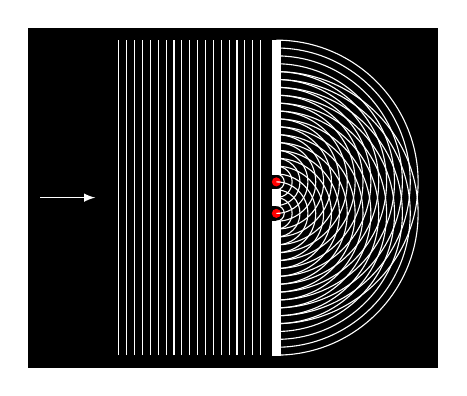
\begin{tikzpicture}[inverted,inverted]
  % direction
  \draw[->] (-3,0) -- +(0.7,0);
  % plain waves
  \foreach\X in {-2,-1.9,...,-0.1} {\draw(\X,-2)--(\X,2);}
  % aperture
  \draw[fill] (0.05,-2) rectangle (-0.05,-0.3);
  \draw[fill] (0.05,-0.1) rectangle (-0.05,0.1);
  \draw[fill] (0.05,2)  rectangle (-0.05,0.3);
  % coordinates
  \coordinate (a) at (0,0.2);
  \coordinate (b) at (0,-0.2);
  % red dots
  \draw[fill,red] (a) circle (0.05);
  \draw[fill,red] (b) circle (0.05);
  % circular waves
  \draw[decoration={expanding waves,angle=90,segment length=0.1cm},decorate] (a) -- +(1.9,0);
  \draw[decoration={expanding waves,angle=90,segment length=0.1cm},decorate] (b) -- +(1.9,0);
\end{tikzpicture}
\end{document}
